The traditional Euclidean notion of dimension cannot adequately describe the complexity and self-similar structure of fractal sets. It becomes necessary to introduce a generalized concept of dimension that extends beyond the integer-valued dimension in classical geometry.\\

The idea becomes clearer when we consider the von Koch curve. Being a curve, its Euclidean dimension is 1 (geometrically one-dimensional). However, due to its fractal nature, the distance along the curve between any two points is infinite.
This highlights the need for a concept of dimension that takes into accounts the fact that the curve occupies "more space" than an ordinary curve, but "less space" than a surface.
\begin{figure}[H]
        \centering
        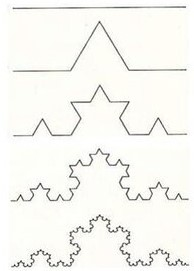
\includegraphics[width=0.35\linewidth]{img/curva di Van Koch.jpg}
        \caption{Creation of the Von Koch curve.}
        %\label{fig:placeholder}
\end{figure}

\subsection{Box-dimension} \label{app:C_Box_dimension}
For this reason is introduced the concept of \textit{box-dimension}. How to obtain the box dimension:
\begin{enumerate}[label=\roman*)]
    \item Cover the whole set with $\varepsilon$-sized boxes (for a set of Euclidean dimension $D$, the covering boxes are $D$-dimensional cubes).
    \item Count the boxes' number $N(\varepsilon)$.
    \item Study the variation of $N(\varepsilon)$ while decreasing $\varepsilon$.
    \item Calculate the Box-dimention.
\begin{equation*}
    d=\lim_{\varepsilon \rightarrow 0} \frac{\ln(N(\varepsilon))}{\ln(1/\varepsilon)}    
\end{equation*}

\end{enumerate}

To simplify, one can say that if $N(\varepsilon)$ scales as $1/\varepsilon^d$ (for a line, $N(\varepsilon) \sim L/\varepsilon$; for a surface, $N(\varepsilon) \sim~A/\varepsilon^2$), then $d$ is the box dimension of the set. This is the case for "well-behaved" fractal sets, such as the Cantor set or the von Koch curve.


\subsection{Correlation dimension} \label{app:C_Correlation_dimension}
When analyzing chaotic systems, the correlation dimension is employed as a measure of fractal dimension, particularly in cases where one works with a set of random points (as in the case study of paragraph \ref{sec:Chaos_BTC}).\\

Compared to the box-counting dimension, the correlation dimension offers several advantages: it can be computed more easily and efficiently, it is less sensitive to noise when only a limited number of points are available, and it often yields results consistent with other dimension estimates (as box-dimension).\\

For any set of $N$ points in a $m$-dimensional space:
\begin{equation*}
    \vb{x}(i)=[x_1(i),\dots,x_m(i)], \quad i=1,2,\dots,N
\end{equation*}
the correlation integral $C(\varepsilon)$ is calculated by:
\begin{equation*}
    C(r)=\lim_{N \to +\infty} \frac{g}{N^2}
\end{equation*}
where $g$ is the number of pairs of points which have a distance between them that is less than distance $r$.\\
As the number of points tends to infinity and the distance between them tends to zero, the correlation integral, for small values of $r$ will take the form 
\begin{equation*}
    C(r) \sim r^\nu
\end{equation*}
where $\nu$ is our correlation dimension.\\
If we have enough points, a log-log graph of the correlation integral vs $r$ will yield an estimate of $\nu$.